\documentclass[12pt]{article}
\usepackage[margin=1.5cm]{geometry}
\usepackage{parskip}
\usepackage{amsmath}
\usepackage{amssymb}
\usepackage{amsfonts}
\usepackage{enumitem}
\usepackage{graphicx}
\usepackage{stmaryrd}
\graphicspath{ {./images/} }


\begin{document}
\begin{enumerate}[label=(\alph*)]
  \item
    Fibbing can induce specific paths in a topology by introducing virtual nodes into the topology that appear to have a very good route to a particular destination, forcing traffic to go along a particular link.

    The diagram below shows what a fibbing controller might do to force a particular path:

    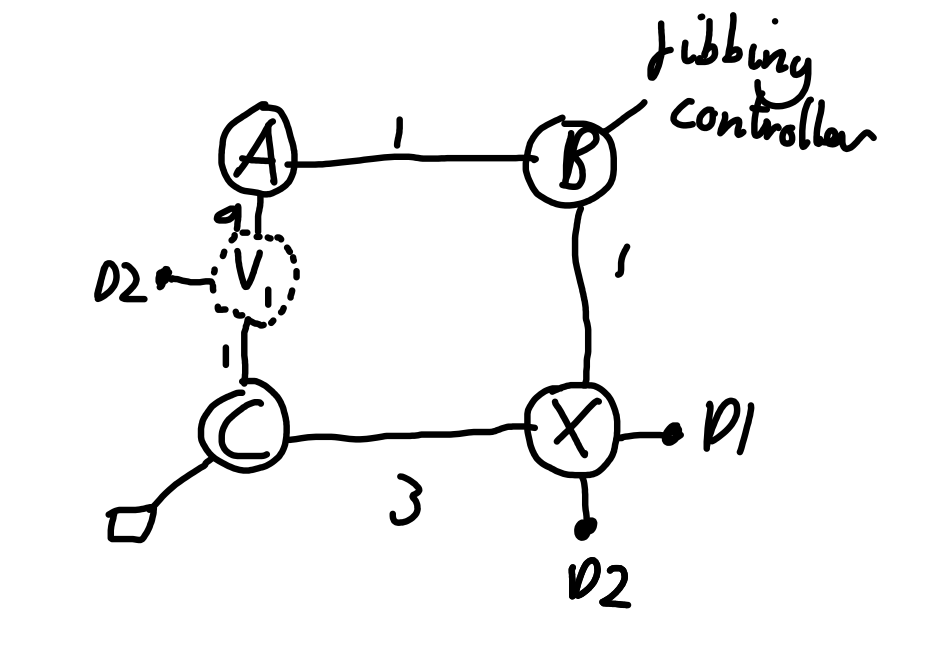
\includegraphics[scale=0.3]{fibbing2}

    In this diagram, we want traffic to be routed along $CABXD_2$ as opposed to $CXD_2$.

    The fibbing controller forces this by introducing a virtual node, $V_1$, that appears to be between $C$ and  $A$ with cost 1, that has an immediate connection to $D_2$. When traffic is actually sent towards $V_1$, because it is on the link between $A$ and $C$, it instead just reaches $A$, where $A$'s best choice is to send it along $ABXD_2$.

    In reality, the fibbing controller might want to insert virtual nodes also between $AB$ and $BX$, forcing the traffic down a particular path, but in this case we do not need to because the topology already results in that behaviour, and in general fibbing controllers will do this removal of virtual nodes when they are not required, called compression.

    The fibbing controller is able to inject this routing information because we use a link-state routing algorithm, which means that topology information is flooded throughout the network, so $B$ will flood the false information throughout the entire network.

  \item
    In the telephone network, we generally never need more than 2 or 3 hops to get from a source to destination. For example, there might be a direct line from London to New York.

    However, telephone traffic is not constant: for example there might be large amounts of load between London and New York on Monday mornings or Friday evenings, and there might not be enough capacity on the direct link to handle all of this traffic.

    In this case, when a link is saturated, we have to choose an alternative path to send extra traffic down that are slightly longer. We might think that since the network is so centralised, and we can gather many statistics, that we should perform some large, complex computations to decide on optimal alternative routes. Instead, we find that a suitable algorithm is just to pick a tandem node $k$, and send excess traffic to $k$, as long as it is operational.

    This algorithm works well due to the randomness properties, which mean that the tandem choices will essentially load balance the traffic by nature.

    We might also implement trunk reservation, to stop small links from getting overwhelmed by traffic from being a tandem. This means that we allocate a particular amount of capacity for a link that can be used as DAR traffic, and do not let traffic exceed this capacity. This ensure that we still have capacity available for normal traffic to keep some level of fairness.


        
\end{enumerate}
\end{document}
